% !TeX program = xelatex
% Lumap System Architecture
% Reproducible build:
%   tectonic Lumap_System_Architecture.tex
\documentclass[11pt,a4paper,fontset=none]{ctexart}

\usepackage[a4paper,margin=22mm,headheight=15pt]{geometry}
\usepackage{fontspec}
\usepackage{amsmath,amssymb,mathtools}
\usepackage{booktabs,tabularx,array,longtable,multirow}
\usepackage{enumitem}
\usepackage{graphicx}
\usepackage{xcolor}
\usepackage{tikz}
\usetikzlibrary{arrows.meta,backgrounds,calc,fit,positioning,shapes.geometric}
\usepackage{fancyhdr}
\usepackage{xurl}
\usepackage{hyperref}
\usepackage{caption}

\IfFontExistsTF{Times New Roman}
  {\setmainfont{Times New Roman}}
  {\setmainfont{TeX Gyre Termes}}
\IfFontExistsTF{Arial}
  {\setsansfont{Arial}}
  {\setsansfont{TeX Gyre Heros}}
\IfFontExistsTF{Menlo}
  {\setmonofont{Menlo}[Scale=0.85]}
  {\setmonofont{Latin Modern Mono}[Scale=0.85]}
\IfFontExistsTF{Songti SC}
  {\setCJKmainfont{Songti SC}}
  {\setCJKmainfont{FandolSong-Regular}}
\IfFontExistsTF{Heiti SC}
  {\setCJKsansfont[AutoFakeBold=2]{Heiti SC}}
  {\setCJKsansfont[AutoFakeBold=2]{FandolHei-Regular}}
\IfFontExistsTF{Hiragino Sans GB}
  {\setCJKmonofont{Hiragino Sans GB}[Scale=0.85]}
  {\setCJKmonofont{FandolFang-Regular}[Scale=0.85]}

\definecolor{LumapBlue}{HTML}{244A73}
\definecolor{LumapLine}{HTML}{66788A}
\definecolor{LumapPale}{HTML}{EFF3F6}
\definecolor{LumapTarget}{HTML}{7A4E22}
\definecolor{LumapGreen}{HTML}{355E4B}
\definecolor{LumapRed}{HTML}{8B3A3A}
\definecolor{LumapGray}{HTML}{555555}

\hypersetup{
  unicode=true,
  colorlinks=true,
  linkcolor=LumapBlue,
  urlcolor=LumapBlue,
  citecolor=LumapBlue,
  pdftitle={Lumap 软件整体架构},
  pdfauthor={Celestial Frontier},
  pdfsubject={macOS 与 iOS 启发式学习系统架构}
}

\ctexset{
  section={format={\Large\bfseries\sffamily\color{LumapBlue}},beforeskip=1.2em,afterskip=.55em},
  subsection={format={\large\bfseries\sffamily},beforeskip=1em,afterskip=.4em},
  subsubsection={format={\normalsize\bfseries\sffamily},beforeskip=.8em,afterskip=.3em}
}

\setlength{\parindent}{2em}
\setlength{\parskip}{0.25em}
\setlength{\emergencystretch}{2em}
\setlist{nosep,leftmargin=2.1em}
\renewcommand{\arraystretch}{1.28}
\captionsetup{font=small,labelfont=bf,labelsep=quad}

\pagestyle{fancy}
\fancyhf{}
\fancyhead[L]{\small\sffamily Lumap 软件整体架构}
\fancyhead[R]{\small\sffamily Current MVP / Target Architecture}
\fancyfoot[C]{\small\thepage}
\renewcommand{\headrulewidth}{0.4pt}

\newcommand{\code}[1]{\begingroup\urlstyle{tt}\nolinkurl{#1}\endgroup}
\newcommand{\codepath}[1]{\begingroup\urlstyle{tt}\path{#1}\endgroup}
\newcommand{\current}{\textcolor{LumapGreen}{\textbf{当前实现}}}
\newcommand{\target}{\textcolor{LumapTarget}{\textbf{目标架构}}}
\newcommand{\planned}{\textcolor{LumapTarget}{\textbf{规划能力}}}
\newcommand{\risk}{\textcolor{LumapRed}{\textbf{限制}}}
\newcommand{\term}[1]{\textbf{#1}}
\newcolumntype{Y}{>{\raggedright\arraybackslash}X}
\newcolumntype{P}[1]{>{\raggedright\arraybackslash}p{#1}}

\tikzset{
  >=Latex,
  currentbox/.style={draw=LumapBlue,very thick,rounded corners=2pt,fill=white,
    align=center,inner sep=5pt,font=\small\sffamily},
  localbox/.style={currentbox,fill=LumapPale},
  targetbox/.style={draw=LumapTarget,very thick,dashed,rounded corners=2pt,fill=white,
    align=center,inner sep=5pt,font=\small\sffamily},
  storebox/.style={cylinder,shape border rotate=90,aspect=0.23,draw=LumapGreen,
    very thick,fill=white,align=center,inner sep=4pt,font=\small\sffamily},
  actor/.style={draw=black,rounded corners=1pt,fill=white,align=center,
    inner sep=4pt,font=\small\sffamily},
  flow/.style={-{Latex[length=2.2mm]},thick,draw=LumapBlue},
  return/.style={-{Latex[length=2.2mm]},thick,dashed,draw=LumapLine},
  targetflow/.style={-{Latex[length=2.2mm]},thick,dashed,draw=LumapTarget},
  boundary/.style={draw=LumapLine,dash pattern=on 4pt off 2pt,rounded corners=3pt},
  note/.style={font=\scriptsize\sffamily,text=LumapGray,align=left}
}

\title{\bfseries\sffamily Lumap 软件整体架构\\[0.35em]
\large macOS 与 iOS 启发式学习系统的当前实现、信任边界与演进设计}
\author{Celestial Frontier}
\date{版本 1.0 \quad 2026 年 9 月 30 日}

\begin{document}
\maketitle

\begin{abstract}
本文给出 Lumap 的软件整体架构，依据仓库中 macOS 0.1.0 与 iOS 0.2.0 的实际代码建立当前实现基线，并将个性化推荐、真实空间计算、跨设备同步等后续能力标为目标架构。文档采用可复现的 XeLaTeX 排版，所有架构图均由 TikZ 生成。当前应用是本地优先的 SwiftUI/SwiftData 产品：两端共享模型、业务状态、供应商客户端和语音服务；API 密钥保存在各自 Keychain；17 种学习方法通过统一完成合同写入活动证据；Narrated Deck 可调用用户配置的远程模型并在失败时明确回退到本地确定性课件；Kokoro 与 sherpa-onnx 在设备上生成旁白；空间学习当前保留可交互的 2D fallback。目标 Recommendation Plane 仅在本文中定义接口与约束，尚未部署为在线策略服务。
\end{abstract}

\noindent\textbf{关键词：}启发式学习；SwiftUI；SwiftData；个性化推荐；离线优先；Kokoro；ARKit；信任边界

\vspace{0.8em}
\noindent\fcolorbox{LumapLine}{LumapPale}{%
  \parbox{0.955\linewidth}{\small
  \textbf{阅读约定。}图中的\textcolor{LumapBlue}{实线框和实线箭头}表示当前仓库已存在的组件或运行路径；\textcolor{LumapTarget}{棕色虚线框和虚线箭头}表示目标组件或尚待实现的链路。架构事实截止到本文版本日期。}}

\tableofcontents
\clearpage

\section{范围、目标与事实基线}

\subsection{设计目标}
Lumap 面向全年龄、多学科和多种表达方式的学习者。系统的工程目标不是把所有学习都交给一个远程模型，而是建立一个可以验证、可以降级并且允许学习者纠正的闭环：输入学习意图，选择学习方法，产生可保存的学习证据，选择是否进行理论或实践检测，再以这些结果调整后续建议。

架构遵循以下原则：
\begin{enumerate}
  \item \term{本地可运行}：创建目标、17 种活动、进度、奖励和 Persona 不依赖网络。
  \item \term{用户意图优先}：用户明确输入的学习主题高于画像推断和推荐结果。
  \item \term{证据分层}：接触、练习、检测与长期保持分别记录，不把一次点击当作掌握。
  \item \term{能力可替换}：远程模型、语音引擎和空间 renderer 均通过边界接口进入，不直接拥有数据库写权限。
  \item \term{降级可见}：网络、语音包或 AR 能力缺失时展示真实状态，不把样例输出冒充在线结果。
  \item \term{当前与目标分离}：运行中的确定性推荐与未来 Recommendation Plane 使用不同状态标签和事件合同。
\end{enumerate}

\subsection{当前工程基线}
\begin{table}[htbp]
\centering
\small
\caption{当前代码基线}
\begin{tabularx}{\textwidth}{P{27mm}P{37mm}Y}
\toprule
维度 & 当前值 & 说明 \\
\midrule
客户端 & macOS 14+，iOS 18+ & 原生 SwiftUI；分别使用 \code{com.local.lumap} 与 \code{com.local.lumap.ios}。 \\
语言与并发 & Swift 6 & 工程启用主 actor 默认隔离；语音引擎池使用独立 actor 串行化推理。 \\
本地存储 & SwiftData & 当前每个应用容器包含一个本地 \code{Lumap} store；尚未实现多档案物理隔离和版本迁移计划。 \\
密钥 & Keychain & 服务名为 \code{com.local.lumap.provider}；密钥不写入 SwiftData、日志或仓库。 \\
学习活动 & 17 种 renderer & 各方法有独立交互案例，完成后写 \code{ActivityRecord}。 \\
远程生成 & 可选 & 支持 OpenAI Chat、Responses 与 Anthropic Messages 形状；当前只有 Narrated Deck 接入生成。 \\
本地语音 & 可选真实推理 & sherpa-onnx 1.13.8 与 Kokoro multilingual v1.1；语音包缺失时进入 silent preview。 \\
空间学习 & 跨端原型 & iOS 检测 ARKit 世界跟踪能力；当前学习 renderer 始终提供 Camera Off 的 2D 交互效果。 \\
推荐策略 & 确定性批次 & 三批本地候选可刷新；LumaPath-RL 尚未训练或部署。 \\
\bottomrule
\end{tabularx}
\end{table}

\subsection{非目标与明确边界}
当前版本没有跨设备账户同步、云端用户数据库、真实社交平台爬取、长期系统级屏幕监测、在线 RL 策略服务或 visionOS target。iOS 的 ARKit capability 检查不等于已有真实相机 AR renderer；公开主页输入当前仅生成本地确定性兴趣预览。未来 Apple 空间设备只能通过公开 SDK 和显式 target 接入，本文不以未发布硬件作为依赖。

\section{当前运行架构}

图~\ref{fig:current-runtime}描述已经存在的主要代码路径。两端共享 \code{LumapStore}、SwiftData 模型、\code{LumapAIClient}、Narrated Deck 合同、Keychain 包装器和 Kokoro 包管理器；平台层分别提供窗口、导航、ARKit capability 与音频会话适配。

\begin{figure}[htbp]
\centering
\begin{tikzpicture}[x=1cm,y=1cm]
  \node[currentbox,text width=31mm] (macui) at (-4.5,0) {macOS UI\\AppShell / Studio\\Assessment / Persona};
  \node[currentbox,text width=31mm] (iosui) at (4.5,0) {iOS UI\\Mobile Root / Studio\\Progress / Spatial};
  \node[localbox,text width=40mm] (shared) at (0,-2.6) {共享状态与用例\\\code{LumapStore}\\Localization / contracts};

  \node[localbox,text width=31mm] (modules) at (-4.5,-5.4) {Shared Studio\\17 method renderers\\Spatial 2D};
  \node[localbox,text width=31mm] (deck) at (0,-5.4) {Narrated Deck\\Coordinator\\schema validation};
  \node[localbox,text width=31mm] (services) at (4.5,-5.4) {Shared Services\\AI client / Keychain\\voice-pack manager};
  \node[currentbox,text width=29mm] (remote) at (8.15,-5.4) {External Model Provider\\HTTPS / user config\\Narrated Deck only};

  \node[storebox,text width=27mm] (db) at (-4.5,-8.35) {SwiftData\\9 类当前模型};
  \node[localbox,text width=31mm] (assets) at (0,-8.35) {本地受保护资产\\Keychain secret\\Kokoro voice pack};
  \node[currentbox,text width=31mm] (spatial) at (-4.5,-11.15) {Spatial capability\\iOS ARKit check\\2D fallback renderer};
  \node[currentbox,text width=31mm] (audio) at (0,-11.15) {sherpa-onnx actor\\24 kHz WAV\\AVAudioPlayer};

  \draw[flow] (macui.south) -- (shared.north west);
  \draw[flow] (iosui.south) -- (shared.north east);
  \draw[flow] (shared.south west) -- (modules.north);
  \draw[flow] (shared.south) -- (deck.north);
  \draw[flow] (shared.south east) -- (services.north);
  \draw[flow] (modules.south) -- (db.north);
  \draw[flow] (deck.south west) -- (db.north east);
  \draw[flow] (deck.east) -- (services.west);
  \draw[flow] (services.south west) -- (assets.north east);
  \draw[flow] (services.east) -- (remote.west);
  \draw[flow] (assets.south) -- (audio.north);
  \draw[flow] (modules.west) -- ++(-0.45,0) |- (spatial.west);

  \begin{scope}[on background layer]
    \node[boundary,fit=(macui)(iosui)(shared)(modules)(deck)(services)(db)(assets)(spatial)(audio),
      inner sep=4mm] (deviceboundary) {};
  \end{scope}
  \node[note,anchor=south west] at ($(deviceboundary.north west)+(0,0.08)$) {设备与 App Sandbox 信任域};
\end{tikzpicture}
\caption{当前运行架构。远程模型网关位于设备信任域之外，且只在用户完成供应商配置后参与 Narrated Deck 生成。}
\label{fig:current-runtime}
\end{figure}

\subsection{表现层与状态层}
macOS 入口为 \code{LumapApp}，主窗口使用 \code{AppShellView}。桌面 Persona 由 \code{MenuBarExtra} 与 \code{PersonaPanelController} 提供。iOS 入口为 \code{LumapiOSApp}，采用移动端独立视图。两端共享领域模型和主要服务文件。\code{LumapStore} 是当前主线程状态编排器，负责创建目标、推荐批次、活动完成、检测、奖励与学习模式状态，并通过 SwiftData 的 \code{ModelContext} 持久化。

这一结构适合 Hackathon MVP，但 \code{LumapStore} 同时承担 UI 状态、用例编排和持久化写入。目标版本应将可测试用例与 Repository 移入 actor，UI 仅消费不可变快照，见第~\ref{sec:evolution}节。

\subsection{持久化模型}
当前 SwiftData schema 包含九类模型。档案与来源层包括 \code{LearnerProfile}、\code{SourceRecord} 和 \code{InterestEvidence}；学习执行层包括 \code{LearningGoal}、\code{ActivityRecord} 与 \code{AssessmentRecord}；其余是 \code{RewardEntry}、\code{MaterialRecord} 与 \code{AppHealthRecord}。核心关联使用稳定 UUID。活动和检测分别用 \code{goalID} 关联目标；奖励使用 \code{eventKey} 保证同一事件不重复入账。

对目标 $g$，MVP 进度由首次出现的不同活动方法、理论检测与实践检测离散推进。可将当前逻辑写为
\begin{equation}
  p_g = \min\!\left(1,\; \frac{|M_g| + I_g^{\mathrm{theory}} + I_g^{\mathrm{practical}}}{5}\right),
  \label{eq:mvp-progress}
\end{equation}
其中 $M_g$ 是目标 $g$ 下已完成且按方法去重的集合，$I$ 是是否存在相应完成证据的指示量。式~\eqref{eq:mvp-progress}只是演示进度投影，不等同于概念掌握概率。

\subsection{17 种学习方法的组件合同}
当前方法枚举包含引导讲解、示例拆解、苏格拉底对话、类比、概念图、分支剧情、闪卡回忆、反向讲解、互动模拟、Spatial AR、刻意练习、反思、误区诊断、好奇分支、反事实实验、迁移挑战和 Narrated Deck。各 renderer 保留自己的输入状态和交互语义，但最终通过共同合同提交：
\begin{equation}
  \operatorname{complete}(g,m,a,h,k)
  \longrightarrow
  \bigl(\texttt{ActivityRecord},\;\texttt{RewardEntry?},\;p'_g\bigr),
\end{equation}
其中 $g$ 为目标，$m$ 为方法，$a$ 为学习产出文本，$h$ 为帮助程度，$k$ 为幂等事件键。当前写入由应用层同步协调；目标 Repository 应把活动、奖励与待投影事件置于同一逻辑事务。

\section{端到端数据流与信任边界}

\subsection{一次学习会话的数据路径}
图~\ref{fig:trust-flow}从输入到证据展示给出完整路径。网络生成只是一条可选分支；本地创建目标、活动交互、保存证据和查看进度不需要远程服务。

\begin{figure}[htbp]
\centering
\begin{tikzpicture}[x=1cm,y=1cm]
  \node[actor,text width=28mm] (learner) at (-5.1,0) {学习者\\明确输入与操作};
  \node[localbox,text width=30mm] (validate) at (-0.75,0) {输入校验\\主题 / 文件类型\\URL / 长度};
  \node[localbox,text width=30mm] (goal) at (3.6,0) {创建或恢复\\LearningGoal\\固定 materialID};

  \node[localbox,text width=30mm] (personal) at (-5.1,-2.7) {Personal\\进度与轨迹\\用户可见};
  \node[localbox,text width=30mm] (evidence) at (-0.75,-2.7) {写入证据\\Activity / Assessment\\Reward 幂等};
  \node[localbox,text width=30mm] (method) at (3.6,-2.7) {运行学习方法\\17 个本地模块\\可选 Deck 生成};

  \node[storebox,text width=28mm] (localdb) at (-5.1,-5.55) {SwiftData\\设备本地};
  \node[storebox,text width=28mm] (secret) at (-0.75,-5.55) {Keychain\\API secret};
  \node[currentbox,text width=31mm] (gateway) at (7.55,-5.55) {外部模型网关\\HTTPS trust boundary\\text / error response};

  \draw[flow] (learner) -- (validate);
  \draw[flow] (validate) -- (goal);
  \draw[flow] (goal.south) -- (method.north);
  \draw[flow] (method) -- (evidence);
  \draw[flow] (evidence) -- (personal);
  \draw[flow] (evidence.south west) -- (localdb.north east);
  \draw[flow] (personal.south) -- (localdb.north);
  \draw[flow] (secret.north east) -- (method.south west);
  \draw[flow] (method.south east) -- (gateway.north west);
  \draw[return] (gateway.west) -- ++(-0.55,0) |- (method.east);

  \begin{scope}[on background layer]
    \node[boundary,fit=(learner)(validate)(goal)(method)(evidence)(personal)(localdb)(secret),inner sep=4mm,
      label={[note]above left:本地受控处理域}] {};
  \end{scope}
\end{tikzpicture}
\caption{端到端学习数据流。密钥仅从 Keychain 进入认证头，不写入生成 prompt 或学习记录。}
\label{fig:trust-flow}
\end{figure}

远程分支只发送主题、可选资料摘录、教学语言和精简学习者上下文；API secret 仅进入 HTTPS 认证头。

\subsection{数据分类与最小披露}
\begin{table}[htbp]
\centering
\small
\caption{数据分类、位置与出域条件}
\begin{tabularx}{\textwidth}{P{30mm}P{34mm}Y P{31mm}}
\toprule
数据 & 默认位置 & 可否发送到远程模型 & 控制 \\
\midrule
学习目标与语言 & SwiftData / 内存 & Narrated Deck 配置后发送 & 用户主动开始生成 \\
资料摘录 & SwiftData 中的限额 excerpt & 仅该课件请求所绑定摘录 & UI 显示来源标签；失败可本地回退 \\
年龄段与背景 & LearnerProfile & 当前可形成精简 learnerContext & 应继续限制字段并提供关闭选项 \\
活动与检测历史 & SwiftData & 当前不发送 & 目标推荐只使用允许列表特征 \\
API 密钥 & Keychain & 仅作为 HTTPS 认证头 & 不进入日志、导出、prompt 或 Git \\
Kokoro 权重与 WAV & Application Support / 临时目录 & 不发送 & 语音在设备上合成，临时 WAV 播放后删除 \\
AR 相机帧 & 当前不采集 & 当前不发送 & 2D fallback 明示 Camera Off \\
\bottomrule
\end{tabularx}
\end{table}

远程生成请求的允许内容集合记为 $A$，用户当前授权集合记为 $C_t$，实际出域字段必须满足
\begin{equation}
  X_{\mathrm{remote},t} \subseteq A \cap C_t,
  \qquad
  \texttt{secret} \notin X_{\mathrm{remote},t}.
  \label{eq:min-disclosure}
\end{equation}
授权撤回或目标 revision 改变后，尚未落库的响应必须失效。当前 MVP 已隔离 Keychain 与 SwiftData，但完整 consent revision 和请求注册表属于目标架构。

\subsection{威胁面与控制}
\begin{longtable}{P{31mm}P{50mm}P{70mm}}
\caption{主要威胁与控制}\label{tab:threats}\\
\toprule
威胁 & 影响 & 控制与剩余工作 \\
\midrule
\endfirsthead
\toprule
威胁 & 影响 & 控制与剩余工作 \\
\midrule
\endhead
恶意资料中的指令 & 模型把资料当系统指令 & Deck adapter 明确要求把 source material 当数据，响应仅接受固定 schema；仍需在生产环境加入内容限额与审计。 \\
伪造或越界模型响应 & UI 崩溃、错误 Quiz & 校验 schemaVersion、3-8 页、连续页码、视觉枚举、强度范围、Quiz 选项与正确答案。 \\
凭据泄漏 & 账户费用和数据风险 & Keychain 存储，设置快照不含密钥，请求只用认证头；发布前补充日志脱敏测试和重定向策略测试。 \\
重复完成或重放 & 奖励重复、进度失真 & \code{RewardEntry.eventKey} 与活动查询去重；目标事件层应加入 sequence 和 requestID。 \\
损坏语音包 & 崩溃或加载任意文件 & 只复制白名单、拒绝符号链接和特殊文件、验证模型与 voices 文件大小；归档 SHA-256 由安装脚本验证。 \\
迟到异步结果 & 覆盖新主题或撤回后的数据 & 语音已支持取消回调；远程生成目标需进一步携带 profile/goal/input revision 并在提交前核对。 \\
\bottomrule
\end{longtable}

\section{Narrated Deck 与本地语音管线}

\subsection{远程生成和确定性回退}
Deck 请求使用版本化的 \code{NarratedDeckGenerationRequest}，包含主题、可选资料摘录及来源标签、语言、精简学习者上下文和最大页数。远程响应必须解码为 \code{NarratedDeckGenerationResponse}，每页包含稳定 ID、标题、2-4 个要点、讲稿、受支持视觉类型和可选 Quiz。图~\ref{fig:deck-sequence}给出当前顺序。

\begin{figure}[htbp]
\centering
\resizebox{0.98\textwidth}{!}{%
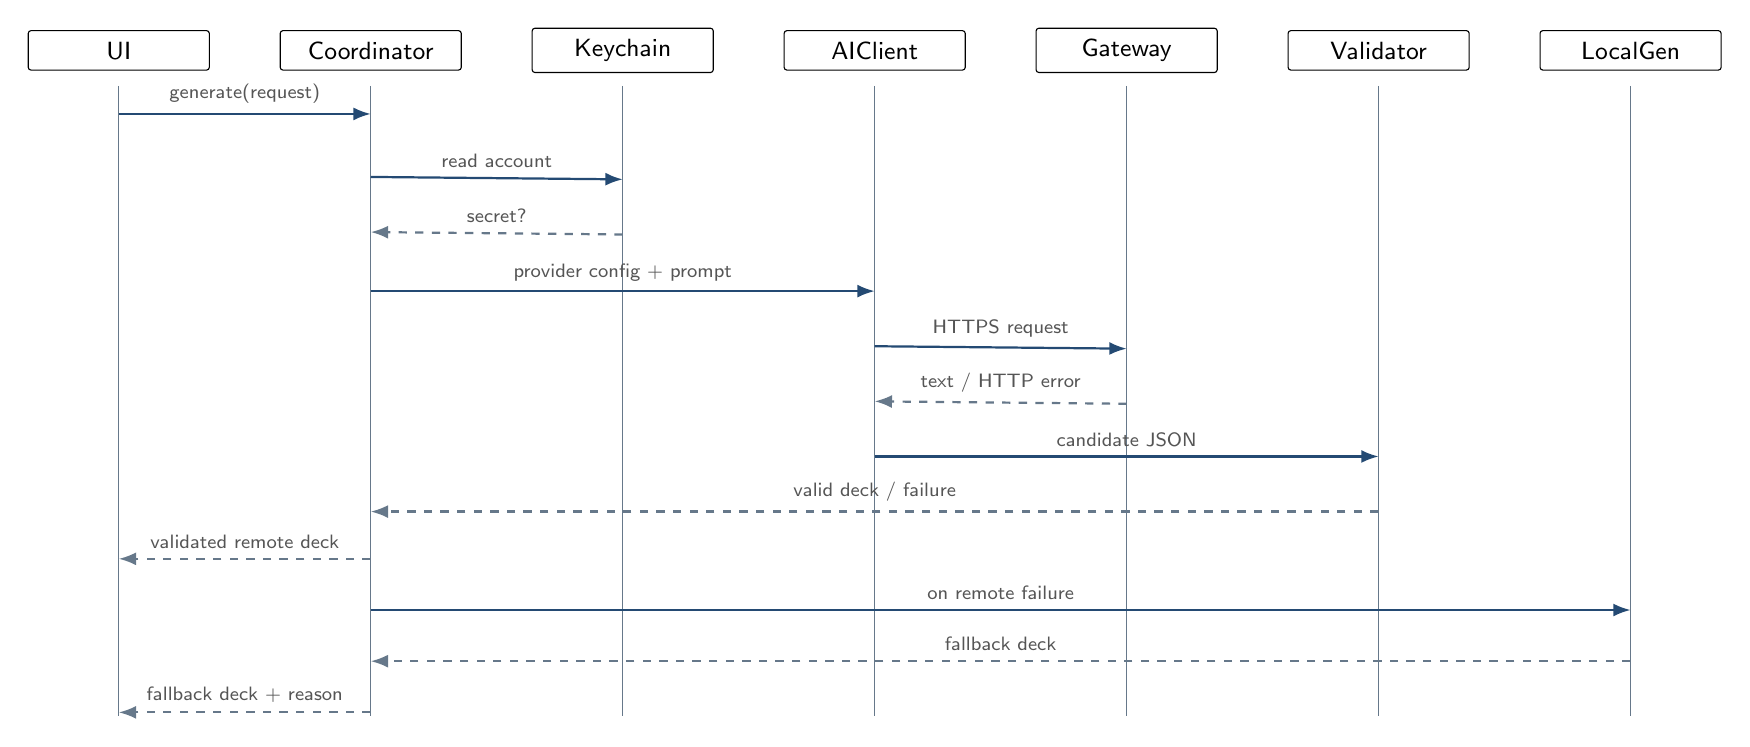
\begin{tikzpicture}[x=1cm,y=1cm]
  \foreach \name/\x in {UI/0,Coordinator/3.2,Keychain/6.4,AIClient/9.6,Gateway/12.8,Validator/16.0,LocalGen/19.2} {
    \node[actor,minimum width=23mm] (\name) at (\x,0) {\name};
    \draw[LumapLine] (\x,-0.45) -- (\x,-8.45);
  }
  \draw[flow] (UI.south) ++(0,-0.55) -- node[above,note]{generate(request)} ($(Coordinator.south)+(0,-0.55)$);
  \draw[flow] ($(Coordinator.south)+(0,-1.35)$) -- node[above,note]{read account} ($(Keychain.south)+(0,-1.35)$);
  \draw[return] ($(Keychain.south)+(0,-2.05)$) -- node[above,note]{secret?} ($(Coordinator.south)+(0,-2.05)$);
  \draw[flow] ($(Coordinator.south)+(0,-2.8)$) -- node[above,note]{provider config + prompt} ($(AIClient.south)+(0,-2.8)$);
  \draw[flow] ($(AIClient.south)+(0,-3.5)$) -- node[above,note]{HTTPS request} ($(Gateway.south)+(0,-3.5)$);
  \draw[return] ($(Gateway.south)+(0,-4.2)$) -- node[above,note]{text / HTTP error} ($(AIClient.south)+(0,-4.2)$);
  \draw[flow] ($(AIClient.south)+(0,-4.9)$) -- node[above,note]{candidate JSON} ($(Validator.south)+(0,-4.9)$);
  \draw[return] ($(Validator.south)+(0,-5.6)$) -- node[above,note]{valid deck / failure} ($(Coordinator.south)+(0,-5.6)$);
  \draw[return] ($(Coordinator.south)+(0,-6.2)$) -- node[above,note]{validated remote deck} ($(UI.south)+(0,-6.2)$);
  \draw[flow] ($(Coordinator.south)+(0,-6.85)$) -- node[above,note]{on remote failure} ($(LocalGen.south)+(0,-6.85)$);
  \draw[return] ($(LocalGen.south)+(0,-7.5)$) -- node[above,note]{fallback deck} ($(Coordinator.south)+(0,-7.5)$);
  \draw[return] ($(Coordinator.south)+(0,-8.15)$) -- node[above,note]{fallback deck + reason} ($(UI.south)+(0,-8.15)$);
\end{tikzpicture}}
\caption{Narrated Deck 当前生成时序。回退结果带有来源说明，不能冒充实时远程生成。}
\label{fig:deck-sequence}
\end{figure}

远程结果的接受条件可以形式化为谓词
\begin{align}
  \operatorname{ValidDeck}(d) ={}& [d.v=v_0]\land[3\le |d.slides|\le 8] \\
  &\land\bigwedge_{i=1}^{|d.slides|}[d_i.index=i]
  \land[d_i.visual\in\mathcal V]
  \land[0\le d_i.intensity\le1] \\
  &\land\bigwedge_{q\in d.quiz}[q.correctID\in q.optionIDs],
\end{align}
其中 $\mathcal V$ 是编译期允许的视觉枚举。若谓词为假、HTTP 失败、密钥缺失或供应商不可用，Coordinator 使用固定模板的 \code{LocalNarratedDeckGenerator} 并保留失败原因供 UI 展示。

\subsection{Kokoro 音频路径}
语音实现不调用系统 TTS。\code{SherpaKokoroEnginePool} 是进程级 actor，缓存一个重量级 sherpa-onnx 引擎并串行化推理；生成回调读取线程安全取消标记，从而允许换页和停止操作中断合成。有效音频保存为 24 kHz WAV，经 \code{AVAudioPlayer} 播放并在停止、完成或失败后清理临时文件。iOS 另设置 spoken-audio 音频会话并处理系统中断。

语音包放在 App Sandbox 的 Application Support 下。macOS 可由固定脚本预装；iOS Settings 允许用户选择已经解压的目录，导入器验证必需文件、拒绝符号链接并先写 staging，再原子替换旧包。语音包缺失或无效时，\code{VoicePackRequiredNarrationProvider} 只推进 silent-preview 时间线、字幕和 Quiz，不产生声音，也不回退到 \code{AVSpeechSynthesizer}。

\section{空间学习与跨端组件}

\subsection{当前 capability 模型}
共享空间协议暴露 availability、scenario、prepare 与 reset；代码类型为 \code{SpatialLearningProviding}。iOS 的 \code{MobileARKitProvider} 在真机检查 ARKit 世界跟踪支持，Simulator 返回 preview-only。macOS 和 iOS 界面都保留可点击的 2D 空间实验。当前 renderer 明确显示 Camera Off / 2D Fallback，因此视觉效果是演示空间交互，不是对真实环境的测量。

\begin{figure}[htbp]
\centering
\resizebox{\textwidth}{!}{%
\begin{tikzpicture}[node distance=8mm and 10mm]
  \node[currentbox,text width=31mm] (sharedsrc) {共享 Swift 源码\\Models / Store\\AI / Voice contracts};
  \node[currentbox,text width=31mm,below left=13mm and 13mm of sharedsrc] (mac) {macOS target\\SwiftUI + AppKit\\Persona NSPanel};
  \node[currentbox,text width=31mm,below right=13mm and 13mm of sharedsrc] (ios) {iOS target\\SwiftUI + UIKit audio\\ARKit capability};

  \node[storebox,text width=28mm,below=12mm of mac] (macstore) {macOS sandbox\\SwiftData / Keychain};
  \node[storebox,text width=28mm,below=12mm of ios] (iosstore) {iOS sandbox\\SwiftData / Keychain};
  \node[localbox,text width=35mm,below=13mm of sharedsrc] (voice) {Kokoro pack per device\\sherpa-onnx shared package};

  \node[currentbox,text width=31mm,below=15mm of macstore] (macfallback) {Desktop simulation\\2D grid / anchors\\Camera Off};
  \node[currentbox,text width=31mm,below=15mm of iosstore] (iosfallback) {Mobile 2D fallback\\capability status\\Camera Off};
  \node[targetbox,text width=37mm,below=15mm of voice] (futurear) {目标空间 renderer\\ARKit / RealityKit\\公开 SDK target};

  \draw[flow] (sharedsrc) -- (mac);
  \draw[flow] (sharedsrc) -- (ios);
  \draw[flow] (mac) -- (macstore);
  \draw[flow] (ios) -- (iosstore);
  \draw[flow] (voice) -- (mac);
  \draw[flow] (voice) -- (ios);
  \draw[flow] (macstore) -- (macfallback);
  \draw[flow] (iosstore) -- (iosfallback);
  \draw[targetflow] (ios) -- (futurear);
  \draw[targetflow] (futurear) -- (iosfallback);

  \node[note,below=6mm of futurear,text width=46mm] {能力或权限不足时继续使用 2D fallback。当前没有云同步；两个容器不会自动交换用户数据或密钥。};
\end{tikzpicture}}
\caption{跨端组件、独立容器与空间能力降级。棕色虚线组件是目标 renderer。}
\label{fig:cross-platform}
\end{figure}

\subsection{目标 renderer 合同}
目标空间层需要把设备能力、权限和运行状态与教学活动分开。接口输入采用版本化 session request，输出带坐标系版本的 \code{Observation}；请求类型为 \texttt{SpatialSession}\allowbreak\texttt{Request}。状态机为
\begin{equation}
  \texttt{checking}\rightarrow
  \left\{
    \begin{array}{ll}
      \texttt{ready}\rightarrow\texttt{tracking}\rightarrow\texttt{paused/stopped}, & \text{能力与权限可用},\\
      \texttt{previewOnly}, & \text{Simulator、拒绝权限或跟踪失败},\\
      \texttt{unavailable}, & \text{无任何 renderer}.
    \end{array}
  \right.
\end{equation}
二维屏幕坐标、相机像素坐标与世界坐标必须使用不同的类型和版本；renderer 只产生 observation，不直接修改掌握度或奖励。

\section{目标 Recommendation Plane}
\label{sec:recommendation}

\subsection{职责边界}
Recommendation Plane 的任务是从允许的候选活动中返回下一步决定及其解释，而不是直接创建数据库记录或绕过安全条件。当前产品只运行确定性推荐批次；本节全部标为\target。推荐服务应支持两类决定：主页发现内容与学习会话内的 concept-method-dose 组合。

\begin{figure}[htbp]
\centering
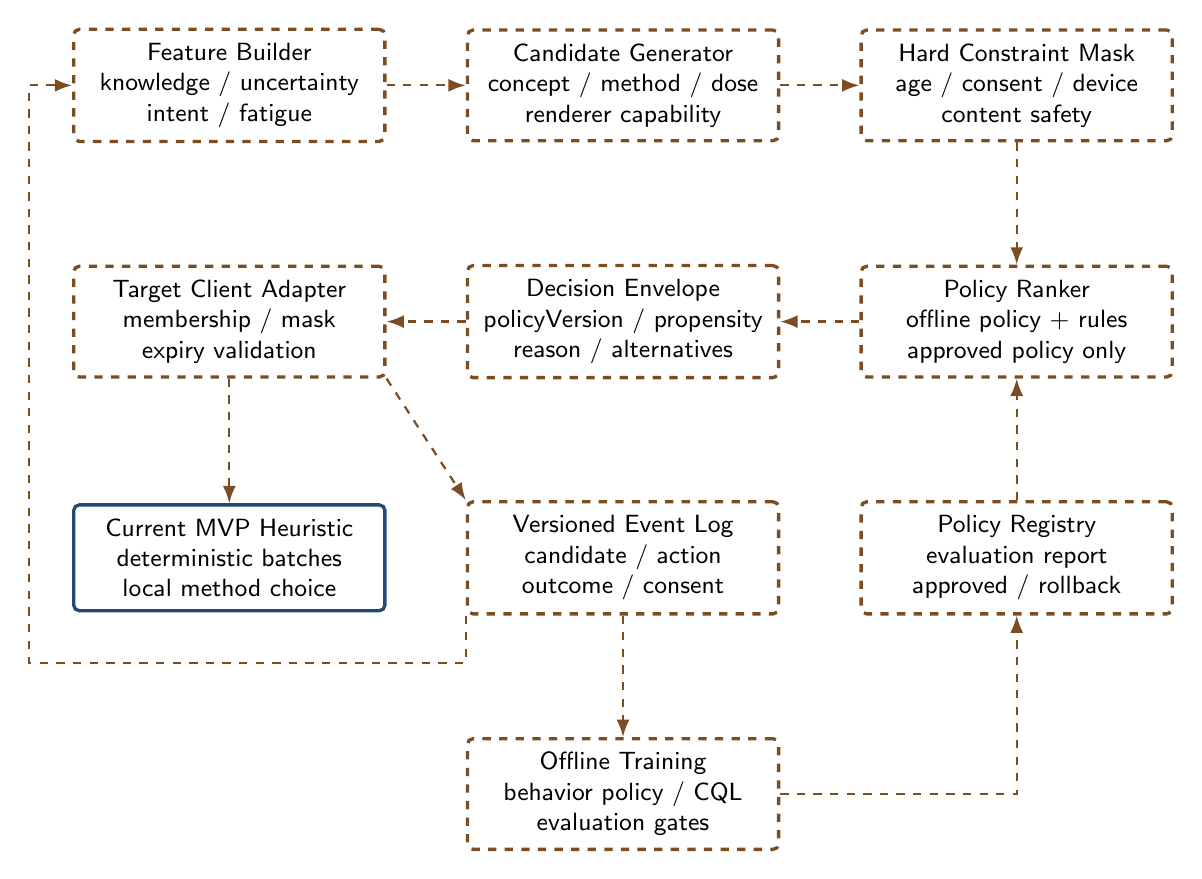
\begin{tikzpicture}[x=1cm,y=1cm]
  \node[targetbox,text width=36mm] (features) at (-5,0) {Feature Builder\\knowledge / uncertainty\\intent / fatigue};
  \node[targetbox,text width=36mm] (candidates) at (0,0) {Candidate Generator\\concept / method / dose\\renderer capability};
  \node[targetbox,text width=36mm] (mask) at (5,0) {Hard Constraint Mask\\age / consent / device\\content safety};

  \node[targetbox,text width=36mm] (client) at (-5,-3.0) {Target Client Adapter\\membership / mask\\expiry validation};
  \node[targetbox,text width=36mm] (decision) at (0,-3.0) {Decision Envelope\\policyVersion / propensity\\reason / alternatives};
  \node[targetbox,text width=36mm] (policy) at (5,-3.0) {Policy Ranker\\offline policy + rules\\approved policy only};

  \node[currentbox,text width=36mm] (heuristic) at (-5,-6.0) {Current MVP Heuristic\\deterministic batches\\local method choice};
  \node[targetbox,text width=36mm] (events) at (0,-6.0) {Versioned Event Log\\candidate / action\\outcome / consent};
  \node[targetbox,text width=36mm] (registry) at (5,-6.0) {Policy Registry\\evaluation report\\approved / rollback};
  \node[targetbox,text width=36mm] (offline) at (0,-9.0) {Offline Training\\behavior policy / CQL\\evaluation gates};

  \draw[targetflow] (features) -- (candidates);
  \draw[targetflow] (candidates) -- (mask);
  \draw[targetflow] (mask.south) -- (policy.north);
  \draw[targetflow] (policy) -- (decision);
  \draw[targetflow] (decision) -- (client);
  \draw[targetflow] (client.south) -- (heuristic.north);
  \draw[targetflow] (client.south east) -- (events.north west);
  \draw[targetflow] (events.south) -- (offline.north);
  \draw[targetflow] (offline.east) -| (registry.south);
  \draw[targetflow] (registry.north) -- (policy.south);
  \draw[targetflow] (events.south west) -- ++(0,-0.6) -| ($(features.west)+(-0.55,0)$) -- (features.west);

\end{tikzpicture}
\caption{目标 Recommendation Plane。棕色虚线组件尚未部署；蓝色实线框是当前确定性 heuristic，也是目标 Adapter 的失败回退。}
\label{fig:recommendation-plane}
\end{figure}

\subsection{状态、候选与决策合同}
学习者状态只从已授权的允许列表特征构造：
\begin{equation}
  s_t = \bigl(k_t,u_t,e_t,m_t,i_t,f_t,q_t,g_t,c_t\bigr),
\end{equation}
分别表示知识估计、不确定性、参与度、方法偏好、明确意图、疲劳、证据质量、当前目标和设备能力。候选动作采用层级结构
\begin{equation}
  a_t=(\text{intent},\text{concept},\text{method},\text{dose},\text{content}).
\end{equation}
在策略打分之前，硬约束 $H(s_t,a)$ 必须形成候选掩码
\begin{equation}
  \mathcal A_t^{\mathrm{safe}}=\{a\in\mathcal A_t\mid H(s_t,a)=1\},
  \qquad
  a_t^*=\arg\max_{a\in\mathcal A_t^{\mathrm{safe}}} Q_\theta(s_t,a).
  \label{eq:safe-action}
\end{equation}
年龄适宜性、授权、设备能力和内容安全属于硬约束，不能被高学习奖励抵消。Decision Envelope 至少包含 \code{decisionID}、动作、候选集哈希、每层 propensity、结构化理由、\code{policyVersion}、\code{consentRevision} 和失效时间。

\subsection{训练、评估与上线闸门}
目标离线训练可采用 Conservative Q-Learning。训练数据先经过硬约束过滤，记为 $D_{\mathrm{safe}}$。一个简化目标为
\begin{align}
\mathcal L_{\mathrm{TD}}(\theta)
 &= \mathbb E_{(s,a,r,s')\sim D_{\mathrm{safe}}}
 \!\left[\left(Q_\theta(s,a)-r-\gamma
 \max_{a'\in\mathcal A^{\mathrm{safe}}(s')}Q_{\bar\theta}(s',a')\right)^2\right],\\
\mathcal L_{\mathrm{CQL}}(\theta)
 &= \mathcal L_{\mathrm{TD}}(\theta)
 +\alpha\,\mathbb E_{s\sim D_{\mathrm{safe}}}
 \left[\log\!\sum_{a\in\mathcal A^{\mathrm{safe}}(s)}e^{Q_\theta(s,a)}
 -\mathbb E_{a\sim D_{\mathrm{safe}}(\cdot|s)}Q_\theta(s,a)\right].
\end{align}
总体奖励可以组合即时掌握增益、延迟保持、迁移、自主性和目标进展，同时扣除挫败、过载、无效重复和提示依赖：
\begin{equation}
 r_t=\sum_i w_i r_{i,t},
 \quad
 J_{C_j}(\pi)=\mathbb E_\pi\!\left[\sum_{t=0}^{T}\gamma^t c_{j,t}\right]\le d_j.
\end{equation}
隐私、年龄、授权和内容安全由式~\eqref{eq:safe-action}的 hard mask 处理。CMDP 只在合法动作集合内约束疲劳、过载和打扰等累积软风险，不能放宽任何硬约束。上线前需要离线策略评估、年龄和语言分层、覆盖率、最差分位表现、fallback 率、人工红队与可回滚 policy registry。无合法候选、超时、签名或版本不匹配时必须走版本化 heuristic fallback。

\section{部署拓扑、故障隔离与回退}

\begin{figure}[htbp]
\centering
\begin{tikzpicture}[x=1cm,y=1cm]
  \node[currentbox,text width=38mm] (provider) at (0,0) {可选外部模型 Provider\\HTTPS / user configured\\Narrated Deck only};
  \node[currentbox,text width=38mm] (macapp) at (-4.4,-2.3) {macOS App Sandbox\\UI / Store / Services};
  \node[currentbox,text width=38mm] (iosapp) at (4.4,-2.3) {iOS App Sandbox\\UI / Store / Services};
  \node[localbox,text width=38mm] (maclocal) at (-4.4,-4.8) {macOS 私有容器\\SwiftData / Keychain\\Kokoro / temporary WAV};
  \node[localbox,text width=38mm] (ioslocal) at (4.4,-4.8) {iOS 私有容器\\SwiftData / Keychain\\imported Kokoro pack};

  \draw[flow] (macapp.north east) -- (provider.south west);
  \draw[flow] (iosapp.north west) -- (provider.south east);
  \draw[flow] (macapp.south) -- (maclocal.north);
  \draw[flow] (iosapp.south) -- (ioslocal.north);

  \node[currentbox,text width=38mm] (clients) at (-5,-8.0) {macOS / iOS clients\\local learning loop\\heuristic fallback};
  \node[targetbox,text width=41mm] (recplane) at (0,-8.0) {Recommendation Plane\\feature + candidate\\policy + registry};
  \node[targetbox,text width=41mm] (sync) at (5,-8.0) {可选账户同步平面\\profile encryption\\delete / export / recovery};

  \draw[targetflow] (clients) -- (recplane);
  \draw[targetflow] (recplane) -- (sync);
\end{tikzpicture}
\caption{部署和故障域。上半为相互独立的当前设备容器；下排虚线为目标服务，不能成为本地学习闭环的单点故障。}
\label{fig:deployment}
\end{figure}

\subsection{故障矩阵}
\begin{table}[htbp]
\centering
\small
\caption{故障检测、用户行为与数据保证}
\begin{tabularx}{\textwidth}{P{31mm}P{39mm}Y}
\toprule
故障 & 用户可见回退 & 数据保证 \\
\midrule
SwiftData 打开失败 & 恢复页，允许重试，不进入空应用 & 不删除、不自动创建替代空库 \\
Provider 配置不完整 & 显示未配置，生成本地 Deck & 密钥不离开 Keychain \\
HTTP、网关或合同失败 & 标注 local fallback 及原因 & 无效响应不写活动证据 \\
Kokoro 包缺失/损坏 & silent preview、字幕和 Quiz 保留 & 不调用系统 TTS，不加载未验证文件 \\
语音合成取消 & 停止或换页立即取消 & 临时 WAV 清理，旧任务不得恢复播放 \\
iOS 音频中断 & 暂停，按系统恢复标志决定是否续播 & playback state 与真实播放器一致 \\
AR 不支持/拒绝权限 & 2D spatial preview & 不产生真实世界跟踪结论 \\
目标推荐服务超时 & 版本化 heuristic fallback & 非法或过期 decision 被客户端拒绝 \\
\bottomrule
\end{tabularx}
\end{table}

\subsection{可观测性与服务目标}
当前应用应记录不含个人原文和密钥的本地诊断事件：组件、状态转移、延迟桶、错误类别、fallback 原因与版本。目标 Recommendation Plane 另记录完整候选集合、hard mask、选中概率、policy version 和延迟结果，以支持离线评估。建议的服务目标为：本地目标创建和活动保存 p95 小于 100 ms；本地 UI 交互保持 60 fps；推荐决定服务端 p95 小于 300 ms；任意远程失败在一次请求预算内显式回退。

系统可用性不是各组件可用性的简单乘积，因为本地 fallback 提供替代路径。若远程路径成功概率为 $A_r$、本地回退成功概率为 $A_f$，且两者失败近似独立，则 Deck 生成的功能可用性为
\begin{equation}
  A_{\mathrm{deck}} = A_r + (1-A_r)A_f.
\end{equation}
该式用于说明降级架构价值，不替代真实故障相关性测试。

\section{接口与数据结构}

\subsection{当前关键接口}
\begin{table}[htbp]
\centering
\small
\caption{主要接口及所有权}
\begin{tabularx}{\textwidth}{P{37mm}P{40mm}Y}
\toprule
接口/类型 & 所有者 & 约束 \\
\midrule
\code{LearningMethod} & 共享 Models & 固定 17 个枚举值；renderer 不应只换标题复用同一交互。 \\
\code{LumapStore} & 当前应用层 & 主 actor；承担用例与 UI 状态，后续拆分。 \\
\code{LumapAIClient} & 共享 Services & 解析 endpoint，支持三种 wire style，45 秒超时，响应提取为文本。 \\
Deck generation request & Deck service & \code{NarratedDeckGenerationRequest} 固定 schema version、topic、excerpt、language、context 与 3-8 页上限。 \\
\code{NarrationProviding} & Voice boundary & availability、playbackState、progress、mute 和播放控制。 \\
Spatial provider contract & Spatial boundary & \code{SpatialLearningProviding} 暴露 capability、scenario、prepare、reset；当前不携带真实相机帧。 \\
Voice-pack manager & Local asset boundary & \code{KokoroVoicePackManager} 验证 allowlist、文件类型与关键大小，导入到固定目录。 \\
\bottomrule
\end{tabularx}
\end{table}

\subsection{目标请求信封}
跨 actor 或跨网络的异步用例应携带版本化信封：
\begin{equation}
\begin{aligned}
  E = (&\texttt{requestID},\texttt{profileID},\texttt{profileRevision},\\
       &\texttt{goalID},\texttt{goalRevision},\texttt{consentRevision},\\
       &\texttt{inputRevision},\texttt{createdAt},\texttt{expiresAt}).
\end{aligned}
\end{equation}
结果提交条件为
\begin{equation}
  \operatorname{Commit}(R,E,t)
  \iff \operatorname{ValidSchema}(R)
  \land t<E.expiresAt
  \land \operatorname{Current}(E)
  \land \neg\operatorname{Cancelled}(E.requestID).
\end{equation}
这避免远程课件、推荐或未来 OCR 的迟到结果覆盖学习者已经修改的目标、档案或授权。

\subsection{事件顺序与幂等性}
目标事件格式 \code{ActivityEvent(instanceID, sequence, action, payloadHash)} 要求同一实例的 sequence 单调递增。Repository 对幂等键 $k$ 的写入满足
\begin{equation}
  \operatorname{apply}(k,e)=
  \begin{cases}
    \text{commit}(e), & k\notin K,\\
    \text{no-op}, & k\in K,
  \end{cases}
\end{equation}
其中 $K$ 是已提交事件键集合。重复网络重试、UI 双击和恢复重放因此不会重复奖励或推进进度。

\section{演进架构与交付顺序}
\label{sec:evolution}

\subsection{从 MVP 到可审计客户端}
第一阶段保持界面与 17 个 renderer 不变，将 \code{LumapStore} 中的持久化写入迁至 \code{@ModelActor LumapRepository}，引入 Sendable DTO、事务幂等键和显式 schema migration。每个档案使用独立 store、附件、索引和 Keychain account；备份采用版本化逻辑快照，Keychain 密钥永不导出。

第二阶段为资料导入建立文档、片段与 citation 模型，加入文件生命周期和删除级联；为异步请求加入第 8 节定义的 revision 信封。远程模型调用继续是可选增强，推荐、检测与 Persona 在各自 adapter 通过评审前不共享一个无限权限 prompt。

\subsection{从确定性推荐到 RL shadow}
Recommendation Plane 的交付顺序应为：先记录可重放事件与候选集，再离线生成 decision，随后以 shadow 模式比较 heuristic 与 policy，最终只对满足闸门的流量小比例启用。每次上线绑定不可变 policy version，并保留一键回退到 heuristic。没有 propensity、候选集或 consent revision 的历史事件不得用于无偏策略评估。

\subsection{从 2D 空间演示到真实 renderer}
先在 iOS 真机建立相机会话、权限、跟踪质量和坐标类型测试，再通过共享空间协议的扩展合同注入 RealityKit renderer。跟踪丢失或设备不支持时回到现有 2D 活动；只有真实 session 产生且带坐标系版本的 observation 才能标记为 camera-assisted evidence。新的 visionOS 或未来设备 target 必须等待公开 SDK，并复用同一证据语义。

\subsection{优先级与验收门槛}
\begin{longtable}{P{18mm}P{47mm}P{76mm}}
\caption{建议交付顺序}\label{tab:roadmap}\\
\toprule
阶段 & 主要工作 & 退出条件 \\
\midrule
\endfirsthead
\toprule
阶段 & 主要工作 & 退出条件 \\
\midrule
\endhead
H0 基线 & 当前 macOS/iOS、17 模块、双类检测、Deck、Kokoro、2D spatial & 两端构建；关键单元测试通过；无密钥进入仓库；fallback 状态可见。 \\
H1 数据可靠性 & VersionedSchema、Repository actor、逻辑导出/恢复、资料引用生命周期 & 迁移、磁盘满、崩溃注入、重复事件和删除级联 fixture 全部通过。 \\
H2 个性化观测 & 候选集、曝光、结果、consent revision、方法效果比较 & 事件可重放；用户可查看和删除来源；缺失数据不被当作负反馈。 \\
H3 RL shadow & 离线训练、OPE、policy registry、客户端验证器 & 分层安全门槛通过；shadow 无写权限；随时回退 heuristic。 \\
H4 空间与同步 & 真实 AR renderer、可选账户同步和设备恢复 & 真机权限/中断测试、坐标一致性、端到端删除与恢复通过。 \\
\bottomrule
\end{longtable}

\section{验证策略}

\subsection{构建与单元测试}
当前工程应至少执行 macOS scheme 的完整测试和 iOS Simulator 通用构建。测试覆盖 endpoint 解析、OpenAI Chat/Responses/Anthropic 文本提取、Deck schema 拒绝、Kokoro 包验证、奖励幂等、进度推进、Keychain 无明文序列化和数据库打开失败路径。外部网关连通性属于独立集成测试，不能使本地单元测试依赖真实密钥或计费账户。

\subsection{架构级故障注入}
建议对以下断点进行自动或手动故障注入：HTTP 400/429/500、无响应和非 JSON；模型返回越界页数和错误 Quiz ID；语音包缺文件、大小不符和符号链接；合成中取消与音频中断；SwiftData 打开失败和保存失败；AR Simulator、拒绝权限和跟踪中断；推荐 decision 过期、不在候选集、违反 hard mask 或来自未知 policy version。

\subsection{可访问性与跨端验收}
两端验证英文默认与中英文切换、动态字号、Reduce Motion、键盘或 VoiceOver 路径、窄屏无横向溢出。Narrated Deck 必须在无音频时保留字幕和 Quiz；空间实验在无摄像头时保留完整的 2D 操作；Persona 提示不能阻断学习任务或自动启动外部观察。

\section{结论}
Lumap 当前已经形成一个本地优先、跨 macOS 与 iOS 的可演示闭环。其可信度来自清晰的能力边界：SwiftData 记录学习证据，Keychain 隔离供应商密钥，17 种 renderer 保持不同交互语义，Narrated Deck 的远程输出经过 schema 校验并具有确定性本地回退，Kokoro 在设备上生成拟人旁白，空间活动在真实 AR 尚未接入时明确维持 2D fallback。

下一阶段的核心不是扩大一个通用模型的权限，而是把持久化、事件、授权 revision 和候选集合做成可审计基础，再以 shadow 方式引入 Recommendation Plane。本文的实线/虚线区分应在每次版本更新时同步维护，使架构图继续反映可运行事实，而不是只描述愿景。

\appendix
\section{当前代码映射}
\begingroup
\footnotesize
\begin{longtable}{P{62mm}P{89mm}}
\toprule
路径 & 架构职责 \\
\midrule
\endfirsthead
\toprule
路径 & 架构职责 \\
\midrule
\endhead
\codepath{Lumap/App/LumapApp.swift} & macOS scene、数据库 bootstrap、恢复界面与独立本地 schema。 \\
\codepath{LumapiOS/App/LumapiOSApp.swift} & iOS scene、移动端数据库打开与恢复入口。 \\
\codepath{Lumap/Models/LumapModels.swift} & 九类 SwiftData 模型、17 种 \code{LearningMethod} 与核心枚举。 \\
\codepath{Lumap/Services/LumapStore.swift} & 当前 UI 状态和学习用例编排、推荐、进度、奖励与 Persona。 \\
\codepath{Lumap/Services/LumapAIClient.swift} & provider-neutral generation request、endpoint 解析、认证头和响应提取。 \\
\codepath{Lumap/Services/NarratedDeckService.swift} & Deck 合同、远程/本地生成、校验、Kokoro 引擎池和播放状态。 \\
\codepath{Lumap/Services/LumapKeychainStore.swift} & 当前供应商 API 密钥的 Keychain 读写边界。 \\
\codepath{Lumap/Services/KokoroVoicePackManager.swift} & 语音包固定目录、导入 staging、安全检查与验证。 \\
\codepath{Lumap/Services/SpatialLearningCapability.swift} & 共享空间能力与 scenario 合同。 \\
\codepath{LumapiOS/Services/MobileARKitProvider.swift} & iOS/Simulator 的 ARKit capability 判断。 \\
\codepath{Lumap/Views/LearningMethodModuleView.swift} & macOS 方法 renderer，包括 Deck 和空间演示入口。 \\
\codepath{LumapiOS/Views/MobileNarratedDeckView.swift} & iOS Deck、旁白、Quiz 和语音包状态交互。 \\
\codepath{LumapiOS/Views/MobileSpatialLearningView.swift} & iOS 空间效果和 2D fallback。 \\
\bottomrule
\end{longtable}
\endgroup

\section{图例与编译说明}
本文不依赖网络图片；六张架构图全部由 TikZ 在编译时生成。仓库脚本使用 Tectonic 的 XeTeX 引擎，并自动重复编译以解析目录和交叉引用：

\begin{verbatim}
brew install tectonic
cd Lumap
./Scripts/compile-architecture-pdfs.sh
\end{verbatim}

字体使用 macOS 自带的 Songti SC、Heiti SC、Times New Roman、Arial 与 Menlo。若在非 macOS 环境编译，应把字体声明替换为已安装的等价 CJK 与拉丁字体；公式和 TikZ 图本身不依赖外部资源。

\end{document}
